\documentclass[12pt]{article}

\usepackage[utf8]{inputenc}
\usepackage[T1]{fontenc}
\usepackage[french,english]{babel}
\usepackage{csquotes}
\usepackage{comment}
\usepackage{appendix}
\usepackage{lmodern}
\usepackage{graphicx,xcolor}
\usepackage{array}
\usepackage[margin=2cm]{geometry}
\usepackage{hyperref}
\usepackage{url}
\usepackage{graphicx}
\usepackage{siunitx}
%\usepackage[lofdepth,lotdepth]{subfig}
\renewcommand{\numberline}[1]{#1~}
\setcounter{secnumdepth}{0}

\definecolor{gris}{rgb}{0.3,0.3,0.3}
\definecolor{vert}{rgb}{0.0, 0.7, 0.0}
\hypersetup{
    pdfstartview={FitH},    % fits the width of the page to the window
    %bookmarks=false,
    colorlinks=true,       % false: boxed links; true: colored links
    linkcolor=black,          % color of internal links
    citecolor=blue,        % color of links to bibliography
    filecolor=blue,      % color of file links
    urlcolor=blue,           % color of external links
    frenchlinks=false
}

\usepackage{tikz}
%\usetikzlibrary{arrows,decorations.pathmorphing}
\usepackage{standalone}

\usepackage[labelsep=quad,indention=10pt]{caption}
\usepackage[labelfont=bf,list=true]{subcaption}
\captionsetup[table]{textfont=it,position=top}
\captionsetup[subtable]{textfont=sf}


\usepackage{xspace}

\usepackage{amssymb,amstext,amsmath,amsthm}
\newtheorem{theoreme}{Théorème}
\newtheorem{lemme}[theoreme]{Lemme}
\newtheorem{corollaire}[theoreme]{Corollaire}

\newcommand{\deriv}{\mathrm{d}}
\newcommand{\dsurd}[2]{\frac{\deriv #1}{\deriv #2}}
\newcommand{\inv}{$^{-1}$}
\newcommand{\card}[1]{\text{Card}(#1)}
\newcommand{\inN}[2]{\in[\![#1,#2]\!]}
\newcommand{\bigo}{\mathcal{O}}
\newcommand{\N}{\mathbb{N}}
\renewcommand{\P}{\mathcal{P}}

\newcommand{\cp}{Cops \& Robbers\xspace}
\newcommand{\hr}{Hunter \& Rabbit\xspace}
\newcommand{\hm}{Hunter \& Mole\xspace}
\newcommand{\cad}{c'est-à-dire\xspace}


\begin{document}
\selectlanguage{french}
%----------------------------------------------------------
\begin{titlepage}
\begin{center}

\textsc{\Large Université de Montréal}\\[4cm]
%
\textsc{\LARGE Recherche sur \hm}\\
\textsc{\LARGE Implémentation de \cp}\\[4cm]
%
\textsc{\Large Par}\\
\textsc{\Large }\\
\textsc{\Large Mathilde Prouvost (20164315)}\\
\textsc{\Large }\\[3cm]
%
\textsc{\Large Bac Sc. Mathématiques et Informatique}\\
\textsc{\Large Faculté des Arts et des Sciences}\\[3.5cm]

\textsc{\Large Travail présenté à Sébastien Roy}\\
\textsc{\Large dans le cadre du cours IFT3150}\\
\textsc{\Large Projet d'informatique -- Initiation à la recherche}\\[.2cm] 
\textsc{\Large Supervisée par Gena Hahn}

\vfill

\textsc{\large Automne 2020 - Hiver 2021}

\end{center}
\end{titlepage}
%-----------------------------------------------------------

\begin{abstract}

Les problèmes d'évasion consistent à trouver le nombre minimal de poursuivants nécessaires pour attraper un évadé se déplaçant sur un graphe. 
Alors qu'originalement le projet consistait en de la recherche sur des variantes de ce problème (principalement \cp et \hm), le but de ce projet est finalement d'implémenter une application permettant de visualiser le problème. L'application devra permettre de dessiner un graphe, de le modifier, de positionner des policiers et un voleur et de les faire se déplacer selon les règles.

\end{abstract}

\selectlanguage{english}
\begin{abstract}

In pursuit-evasion problem, the minimal number of cops needed to find a robber on a graph has to be found. The first goal of my project was to do some research around the \cp problem and its variants (especially the \hm problem). But then it changed to the second goal: implement an app to draw a graph to picture \cp strategies.

\end{abstract}
\selectlanguage{french}

\tableofcontents

\section{Introduction : vocabulaire et notations}

\subsection{Les graphes}
Un \emph{graphe} non-orienté $G$ est un couple $(V,E)$ composé de l'ensemble $V$ des \emph{sommets} (ou \emph{noeuds}) et de l'ensemble $E$ des \emph{arêtes} (paires de sommets) tel que $E \subset \{\{u,v\}, (u,v)\in V^2\}$. On note $n=\card{V}$ le nombre de noeuds du graphe. Dans un graphe orienté, les arêtes ne sont pas $\{u,v\}$ mais $(u,v)$, i.e l'ordre importe. On peut aussi noter les arêtes $u \cdot v$ ou plus simplement $uv$.

Un graphe est \emph{simple} si l'ensemble des arêtes ne contient pas de boucle, \cad pour tout $u\in V$, $u \cdot u \notin E$.

Le \emph{graphe trivial} est le graphe simple $(\{u\},\varnothing)$ où $u$ est un sommet unique.

Deux noeuds $u,v$ sont \emph{voisins} si $u\cdot v \in E$. Le \emph{degré} d'un noeud $u$ est le nombre de ses voisins, \cad $\card{\{v\in V, u \cdot v \in E\}}$. Une \emph{feuille} est un sommet de degré 1.

Une \emph{chaîne} $u-v$ entre les noeuds $u$ et $v$ est une séquence de $t$ noeuds voisins \cad $(u_k)_{k\inN{1}{t}}$ avec $u_1=u$, $u_t=v$ telle que $\forall k\inN{1}{t-1},\ u_{k} \cdot u_{k+1} \in E$. $t$ est appelé la \emph{longueur} de ce chemin. Pour un graphe orienté, on parle de \emph{chemin}.

Un \emph{cycle} est une chaîne dont le point d'arrivée est le point de départ (chaîne $u-u$). Pour un graphe orienté, on parle de \emph{circuit}. Le $k$-cycle est le cycle de longueur $k$.

Un graphe est dit \emph{connexe} si pour chaque paire de sommets $(u,v) \in V^2$ telle que $u \neq v$, il existe une chaîne reliant $u$ à $v$.

Un \emph{arbre} est un graphe connexe sans cycle.

\subsection{Les problèmes d'évasion}

Un problème d'évasion est un problème dans lequel sont donnés un graphe, $k$ poursuivants et un évadé. Les $k+1$ personnages sont positionnés sur des noeuds du graphe et peuvent se déplacer selon les arêtes. Le but de l'évadé est de rester sur des noeuds sans poursuivant, alors que les poursuivants doivent attraper l'évadé, \cad être sur le même noeud. Les poursuivants forment une équipe, l'évadé seul une autre. Le jeu va alors être d'alterner les mouvements de chaque équipe. Le problème répond à la question \og Les $k$ poursuivants peuvent-ils attraper l'évadé en un temps fini ? \fg en essayant de trouver des stratégies qui permettent aux poursuivants d'attraper l'évadé ou au contraire des stratégies permettant à l'évadé de s'échapper. 

Il en existe plusieurs variantes en fonction de différents possibilités sur le graphes et les personnages. Par exemple, le graphe peut être orienté ou non, l'ensemble des arêtes peut être différent pour les policiers que pour le voleur, les personnages peuvent avoir un champ de vision restreint du graphe, les personnages peuvent ne pas se déplacer à la même vitesse, les personnages peuvent avoir la possibilité de ne pas bouger à leur tour, les personnages peuvent connaître la stratégie adverse, etc. Le problème général de \cp se situe sur un graphe simple non-orienté. Les poursuivants sont appelés des policiers et l'évadé un voleur. Tous les personnages ont une connaissance entière du graphe. Le problème \hm se différencie du problème \cp par le fait que les poursuivants (chasseurs) peuvent se déplacer sans contrainte du graphe, mais ne connaissent pas la position de l'évadé (taupe ou lapin), qui lui ne peut pas ne pas se déplacer et connaît la stratégie des poursuivants en avance. C'est principalement ce problème que j'ai étudié, à travers les papiers \cite{komarov2013hunter}, \cite{tayy2016evasion}, \cite{abramovskaya2016hunt}, \cite{britnell2012finding} et \cite{guggiari2018approximating}.

La question principale de tous ces problèmes est : en fonction de caractéristiques du graphe, quel est le nombre minimal de poursuivants suffisants pour qu'ils attrapent l'évadé ? Notamment, la conjecture de Meyniel en évalue une borne supérieure sur le problème \cp à $\bigo(\sqrt{n})$.

Un graphe est dit \emph{$n$-Cop-Win} ou \emph{$n$-Hunter-Win} si $n$ poursuivants sont suffisants pour attraper l'évadé pour les problèmes \cp et \hm respectivement \cad s'il existe une stratégie gagnante pour le poursuivant. Si $n=1$, on dit simplement \emph{Cop-Win} et \emph{Hunter-Win}, et on peut employer les termes \emph{Robber-Win} et \emph{Mole-Win} si l'évadé peut s'enfuir, \cad s'il existe une stratégie gagnante pour l'évadé.

\section{Historique de mon travail}

\subsection{\'Etude des problèmes d'évasion avec un unique poursuivant (\cite{komarov2015hunter})}

\subsubsection{\cp avec un unique policier (\cite{nowakowski1983vertex}, 1973)}

Le sommet $u$ \emph{domine} le sommet $v$ si pour chaque noeud $w$ voisin de $v$, $w$ est aussi voisin de $u$. On dit que $v$ est un \emph{coin}.

Un graphe est dit \emph{pliable} s'il contient une séquence de coins qui mènent au graphe trivial.

\begin{figure}[h!]
    \centering
    \includestandalone[]{pliable1}\quad\quad
    \includestandalone[]{pliable2}\quad\quad
    \includestandalone[]{pliable3} \\
    \includestandalone[]{pliable4}\quad\quad
    \includestandalone[]{pliable5}\quad\quad
    \includestandalone[]{pliable6}\quad\quad
    \includestandalone[]{pliable7}
    \label{fig:pliable}
    \caption{\textbf{Exemple de construction d'arbre pliable}}
\end{figure}

\begin{theoreme}
    Pour le problème \cp avec un unique poursuivant, un graphe est cop-win si et seulement s'il est pliable.
\end{theoreme}

\begin{proof}
\boxed{\Leftarrow} Montrons d'abord que le policier gagne sur les graphes pliables.

Soit $G = (V,E)$ un graphe pliable non trivial. Alors par définition, on a une suite $(u_k)_{k\inN{0}{n-1}}$ de coins menant au graphe trivial au sommet $u_{n-1}$. On peut alors utiliser les déplacements du policier suivant $(u_{n-1-k})_{k\inN{0}{n-1}}$. A ce moment, le voleur ne pourra pas s'échapper.

En effet, chacun des noeuds visités par le policier ne pourra pas être atteint par le voleur après son passage sans être capturé. On peut supprimer un tel noeud dominé du graphe puisque le voleur ne pourra pas s'y rendre sans être capturé. 

On procède alors par induction descendante pour atteindre le cas de base du graphe trivial.

Le policier gagne sur le graphe trivial, car le voleur ne peut pas se positionner ailleurs que sur le sommet déjà occupé par le policier.

\boxed{\Rightarrow} Maintenant, prouvons que si le policier gagne sur un graphe, alors ce graphe est pliable.

Même s'il joue optimalement, le dernier noeud sur lequel le voleur se place est dominé par le policier, sinon il pourrait continuer à jouer. En enlevant ce noeud, le graphe doit toujours pouvoir être gagné par le policier, sinon le voleur n'emprunterait jamais ce noeud et pourrait gagner. On a trouvé notre premier coin.

On procède alors par induction descendante pour atteindre le cas de base du graphe trivial, qui est bien un graphe pliable.
\end{proof}

\subsubsection{\hm avec un unique chasseur (\cite{komarov2013hunter}, 2019)}

\begin{lemme}\label{thm:sous-graphe}
    Si un graphe $H$ est mole-win, alors tout graphe $G$ ayant $H$ pour sous-graphe est mole-win.
\end{lemme}

\begin{proof}
Si $H$ est mole-win, alors la taupe a une stratégie gagnante sur ce sous-graphe. Il lui suffit de rester sur ce sous graphe pour réussir à échapper au chasseur qui ne pourra donc pas avoir de stratégie gagnante.
\end{proof}

\begin{corollaire}\label{thm:composante-connexe}
    La nature d'un graphe est directement obtenue selon la nature de chacune de ses composantes connexes selon la loi suivante : si une composante est mole-win, alors le graphe est mole-win; sinon le graphe est hunter-win.
\end{corollaire}

\begin{proof}
Si aucune composante connexe n'est mole-win (\cad toutes les composantes sont hunter-win), alors le chasseur devra appliquer sa stratégie gagnante sur chaque composante. Ainsi, quelque soit la composante sur laquelle est la taupe, elle se fera attraper, puisqu'elle ne peut pas changer de composante.

Au contraire, si une composante est mole-win, alors on peut utiliser le lemme \ref{thm:sous-graphe}. La taupe pourra utiliser sa stratégie gagnante pour éviter le chasseur, qu'il tire sur sa composante ou non.
\end{proof}

Dans un arbre, on peut définir une \emph{parité} des noeuds. En effet, puisqu'un arbre est connexe, deux noeuds $u,v$ sont toujours connectés donc il existe un chemin entre eux. Si on n'autorise pas les allers-retours sur un chemin, ce chemin est unique puisqu'un arbre ne contient pas de cycle. On peut donc parler de \emph{la} distance entre deux noeuds car celle-ci est unique. Ainsi, en marquant un sommet quelconque appelé \emph{racine}, l'ensemble des noeuds pairs sera l'ensemble des noeuds situés à une distance paire de la racine et l'ensemble des noeuds impairs est l'ensemble des noeuds situés à une distance impaire de la racine. Par les propriétés de la parité dans $\N$, deux noeuds de même parité ne peuvent pas être voisins.

Un \emph{homard} est un arbre constitué d'un chemin $\P$ (le \emph{chemin principal}) et de noeuds situés à une distance maximale de 2 d'un noeud de $\P$.

Les noeuds à distance 1 du chemin principal sont appelés des \emph{genoux}, les feuilles à distance 2 de ce même chemin des \emph{pieds} et les sommets du chemin principal reliés à des genoux des \emph{hanches}.

\begin{figure}[h!]
    \centering
    \includestandalone[]{lobster1c} \quad\quad
    \includestandalone[]{lobster2c}
    \caption{\textbf{Exemples de homards coloriés selon la parité des noeuds} Les chemins principaux sont horizontaux.}
    \label{fig:lobster}
\end{figure}

\begin{theoreme}\label{thm:lobster}
    Pour le problème \hm avec un unique poursuivant, les homards sont hunter-win.
\end{theoreme}

\begin{proof}
Montrons que le chasseur gagne sur les homards, en explicitant sa stratégie.

Remarquons d'abord que, puisque la taupe doit se déplacer d'une distance exactement 1 à chaque fois, sa position changera de parité à chaque tour.

Sans perte de généralité, on va fixer la racine à une extrémité du chemin principal. On va faire une disjonction de cas, selon si au premier tour la proie est sur un sommet pair ou impair. 

On va d'abord supposer qu'elle est sur un sommet d'une certaine parité et éliminer toutes les possibilités. Si on attrape la taupe, c'est qu'elle était de cette parité. Sinon, c'est qu'elle était sur l'autre parité. Dans ce cas, il faut avoir fait un nombre impair de tour (au besoin, gâcher un tour sans cible apparente) pour se retrouver à la situation initiale avec la taupe dans la bonne parité. Il suffira alors de refaire notre stratégie gagnante pour l'attraper. 

Explicitons notre stratégie gagnante sur une taupe de la bonne parité. Un exemple est illustré à la figure \ref{fig:hunter-win}.

\begin{figure}[]
    \centering
    \includestandalone[]{hunter-win2}\quad\quad
    \includestandalone[]{hunter-win3}\quad\quad
    \includestandalone[]{hunter-win4}\quad\quad
    \includestandalone[]{hunter-win5}\quad\quad
    \includestandalone[]{hunter-win6}\quad\quad
    \includestandalone[]{hunter-win7}\quad\quad
    \includestandalone[]{hunter-win8}
    \caption{\textbf{Stratégie gagnante pour le chasseur} En rouge est la position du chasseur, en vert les positions possibles de la taupe. On a commencé par supposer que la taupe était au tour $t=0$ sur un noeud pair de la même parité de le sommet rouge. Si ce n'était pas le cas, il faut alors refaire la stratégie puisqu'on a joué un tour impair de tours, la taupe qui était à $t=0$ sur un sommet impair est maintenant sur un sommet pair. Si ça n'avait pas été le cas, refaire le tour $t=0$ avant de reprendre à ce même tour une fois supplémentaire permet de changer la taupe de parité. Finalement, la taupe ne peut être sur aucun sommet sans avoir été attrapée.}
    \label{fig:hunter-win}
\end{figure}

En ne se déplaçant que d'une distance 1, le chasseur va changer de parité de la même façon que la taupe. La stratégie consiste à suivre le chemin principal en se déplaçant d'un sommet à son voisin. En présence de genou, il y a deux possibilités : soit le genou n'a pas de pied, soit il en a un. Si le genou n'a pas de pied, puisqu'il n'y a qu'un sommet à un distance impaire dans la branche du genou, la taupe ne peut pas y être, et donc le chasseur continue. Sinon, la taupe peut se trouver dans un pied. Dans ce cas, le chasseur va devoir aller sur le genou. La taupe n'en étant pas à une distance 1 sur le chemin principal, elle ne va pas pouvoir profiter de ce ``détour'' pour aller sur un sommet antérieur du chemin principal. Après cela, si elle était effectivement sur le pied, elle se fait attraper sur le genou, sinon, le chasseur devra repasser par la hanche pour conserver sa parité. En présence de plusieurs pieds sur un même genou, tous les pieds arrivent sur le genou du chasseur. En présence de plusieurs genoux à pied, le chasseur devra éliminer les pieds de chacun séparément, mais puisqu'il ne changera jamais de parité, la taupe ne pourra pas en profiter pour s'échapper.

Après avoir parcouru tout le chemin principal et les genoux, le chasseur aura éliminé toutes les positions possibles pour la taupe. S'il ne l'a pas encore attrapée, c'est qu'elle a débuté sur une parité opposée. En attendant un nombre de tours impair depuis le début, la taupe sera alors sur la bonne parité, et refaire la stratégie assure d'attraper la taupe. 

Ainsi, avec cette stratégie, le chasseur est assuré d'attraper la taupe en un temps fini, quelle que soit la stratégie de la taupe pour essayer de s'enfuir.
\end{proof}

\begin{lemme}\label{thm:cycle}
    Les cycles de taille $n\geq 3$ sont mole-win.
\end{lemme}

\begin{proof}
D'après les règles, la taupe connaît la stratégie du chasseur. Dans un graphe de taille $n\geq3$, tous les sommets sont de degré 2. Si le chasseur tire sur un sommet, la taupe avait au tour d'avant la possibilité d'aller sur l'autre sommet qui était relié à sa position.

En fait, l'impossibilité pour le chasseur d'enfermer la taupe dans un cul-de-sac (chemin qui termine sur des feuilles) permet à la taupe de toujours s'évader.
\end{proof}

\begin{lemme}\label{thm:araignee}
    Le graphe $S_{3,3}$, décrit à la figure \ref{fig:araignee}, est mole-win.
\end{lemme}

\begin{figure}[]
    \centering
    \includestandalone[]{araignee}
    \caption{Le graphe $S_{3,3}$, aussi appelé \emph{araignée à 3 pattes}}
    \label{fig:araignee}
\end{figure}

\begin{proof}
Je ne vais pas expliciter une preuve rigoureuse. Celle-ci est bien écrite dans \cite{komarov2013hunter}. Je vais tout de même en expliquer la principale logique. 

La démonstration consiste en une disjonction de cas décrite par un diagramme d'états fini, qui montre que quelque soit la stratégie du chasseur, la taupe peut s'échapper. Voici quelques résultats tout de même intéressants à noter.

La taupe a ou bien 1 degré de liberté (sur les feuilles), ou bien 2 (au milieu des branches) ou bien 3 (au centre).

Le chasseur peut empêcher la taupe de changer de branche en tirant toujours au centre. Cependant, la taupe a assez de liberté au sein d'une branche pour y rester libre.

Le chasseur peut épuiser les possibilités d'une branche. La taupe pouvait s'assurer de ne pas être sur cette branche précise. En s'acharnant sur une unique branche, le chasseur ne peut pas empêcher la taupe de changer de branche entre temps, en passant par le centre. 

Contrairement à un homard, si on considère deux branches de l'araignée comme le chemin principal, rien n'empêche à la taupe d'être sur la troisième branche. Si ce n'est pas le cas, lorsque le chasseur va essayer d'éliminer les possibilités sur celle-ci, la taupe pourra en profiter pour retourner sur les pas du chasseur et ainsi lui échapper. Puisqu'elle connaît la stratégie du chasseur, elle peut s'arranger initialement pour choisir de ne pas être sur cette branche.

Finalement, il faut retenir que c'est la possibilité de revenir sur des sommets vérifiés et éliminés par le chasseur qui permet à la taupe de s'enfuir.
\end{proof}

\begin{theoreme}
    Un graphe $G$ connexe est hunter-win si et seulement si il est un homard.
\end{theoreme}

\begin{proof}
Montrons le sens direct en cherchant les graphes connexes hunter-win.

Maintenant, si le graphe n'est pas un arbre, il contient un cycle et il est donc mole-win d'après le théorème \ref{thm:cycle}. Ainsi, seuls des arbres peuvent être hunter-win.

Si c'est un arbre qui n'est pas un homard, alors il contient $S_{3,3}$. En effet, il existe un plus long chemin noté $\P$ car le nombre de noeuds de $G$ est borné (par $n$) et dans $\N$. Il existe un noeud $u$ à une distance d'au moins 3 de $\P$, sinon notre graphe serait un homard. En notant $c$ le sommet de $\P$ le plus proche de $u$, il existe deux sommets $v_1,v_2$ à distance 3 de $c$ sur $\P$, sinon $\P$ passerait par $u$ pour être plus long. En utilisant $c$ comme noeud central et les noeuds entre $c$ et $u,v_1,v_2$ pour les branches, on a trouvé un sous-graphe de la forme de $S_{3,3}$. D'après le théorème \ref{thm:araignee}, ce graphe est mole-win. Finalement, seuls les arbres qui sont des homards peuvent être hunter-win.

Finalement, d'après le théorème \ref{thm:lobster}, les homards sont hunter-win, et ce sont les seuls graphes connexes qui le sont.
\end{proof}

\subsection{Implémentation d'une application pour visualiser \cp}

Tout le code est sur mon \href{https://github.com/MathProuv/IFT3150}{GitHub}.

J'ai développé une interface visuelle pour dessiner des graphes et pouvoir jouer aux \cp. J'ai opté pour une Programmation Orientée Objet et une logique Modèle-Vue-Contrôleur. J'ai donc préféré utiliser Java (et JavaFX).

\begin{figure}[h!]
    \centering
    \subcaptionbox{Création du graphe
        \label{screen:graphe}}
        {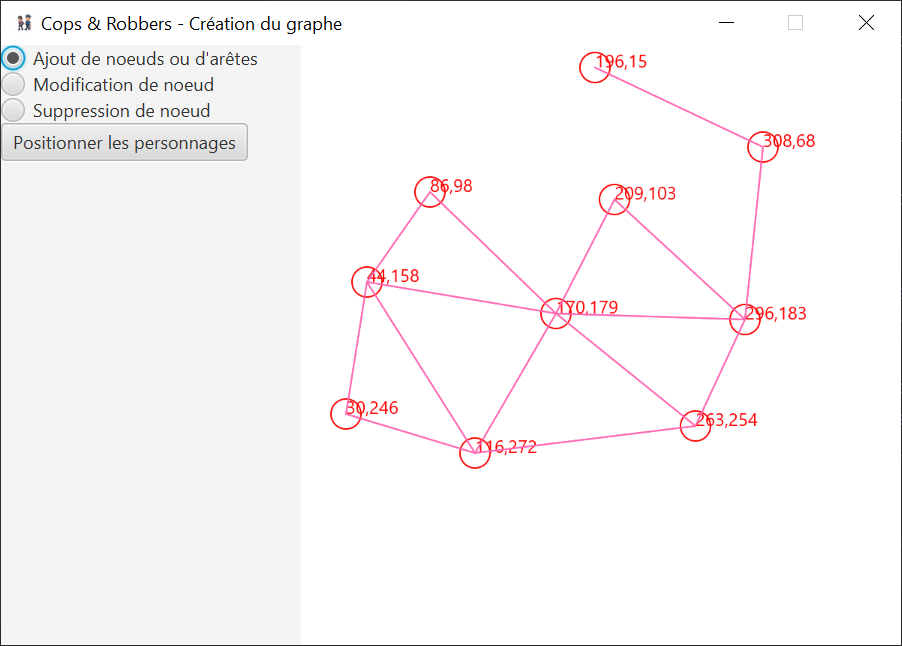
\includegraphics[width=0.45\textwidth]{modif_graphe2.PNG}}
    \subcaptionbox{Positionnement des personnages
        \label{screen:perso}}
        {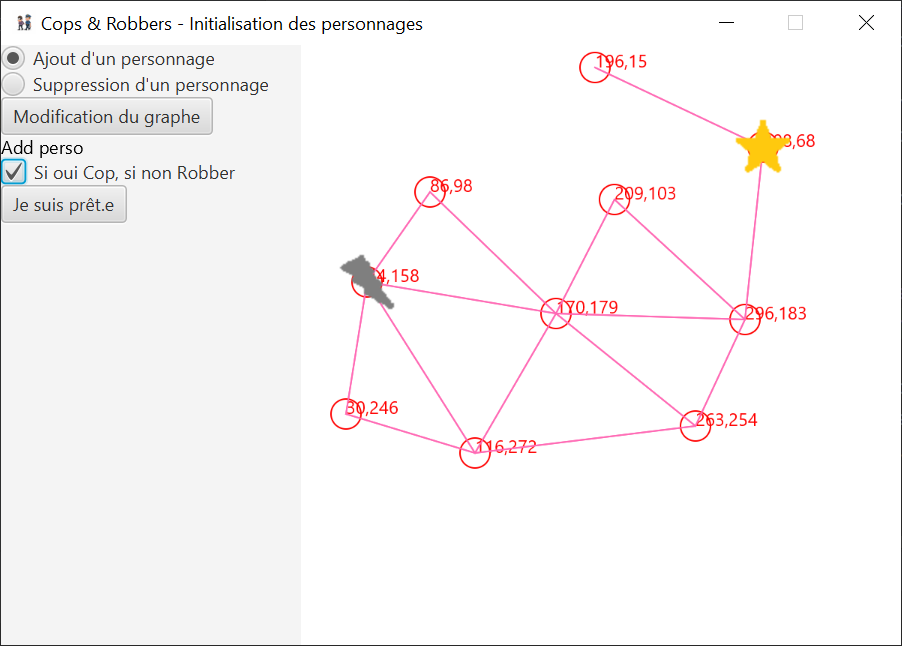
\includegraphics[width=0.45\textwidth]{modif_perso.PNG}}
    \subcaptionbox{Fenêtre de jeu
        \label{screen:jeu}}
        {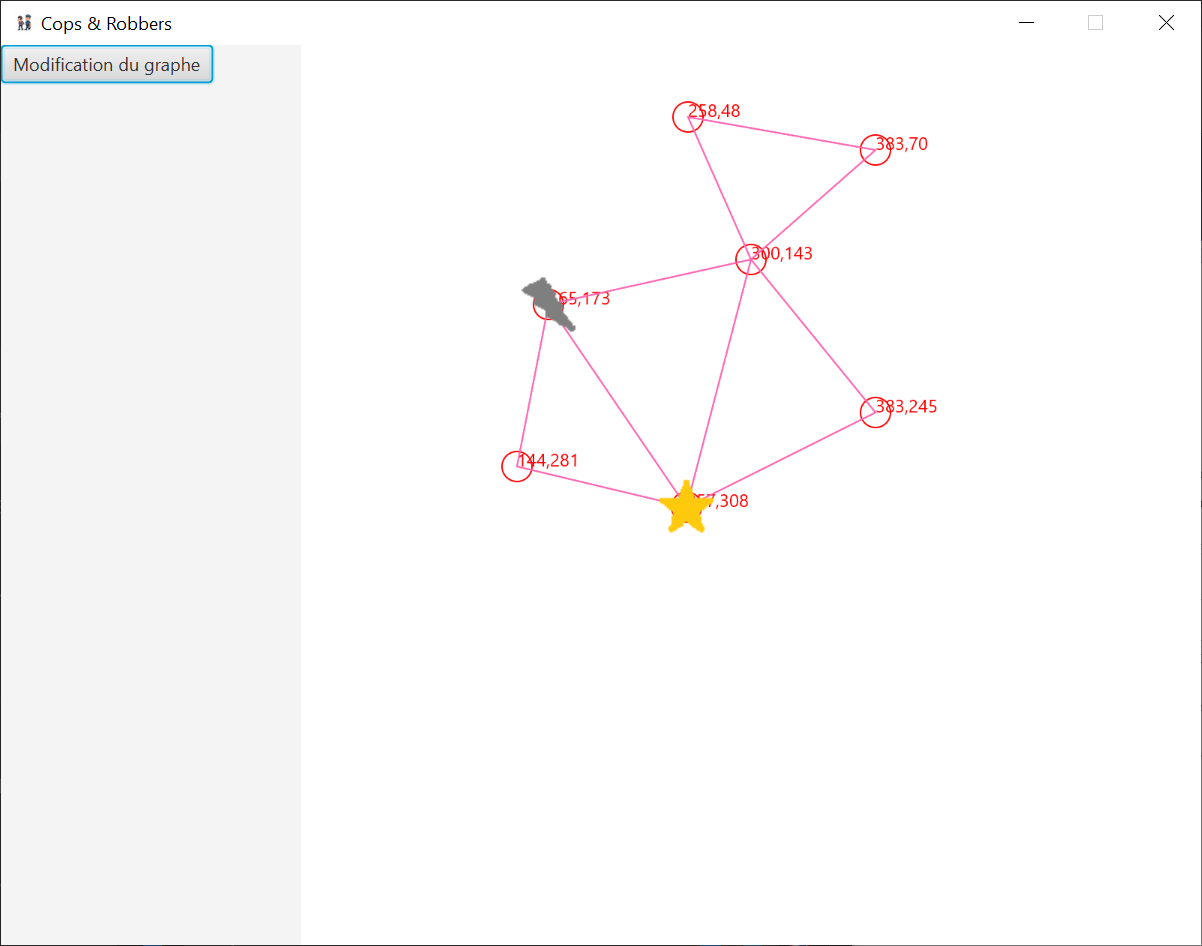
\includegraphics[width=0.45\textwidth]{modif_jeu.PNG}}
    \subcaptionbox{Fenêtre de ré-initialisation
        \label{screen:perdu}}
        {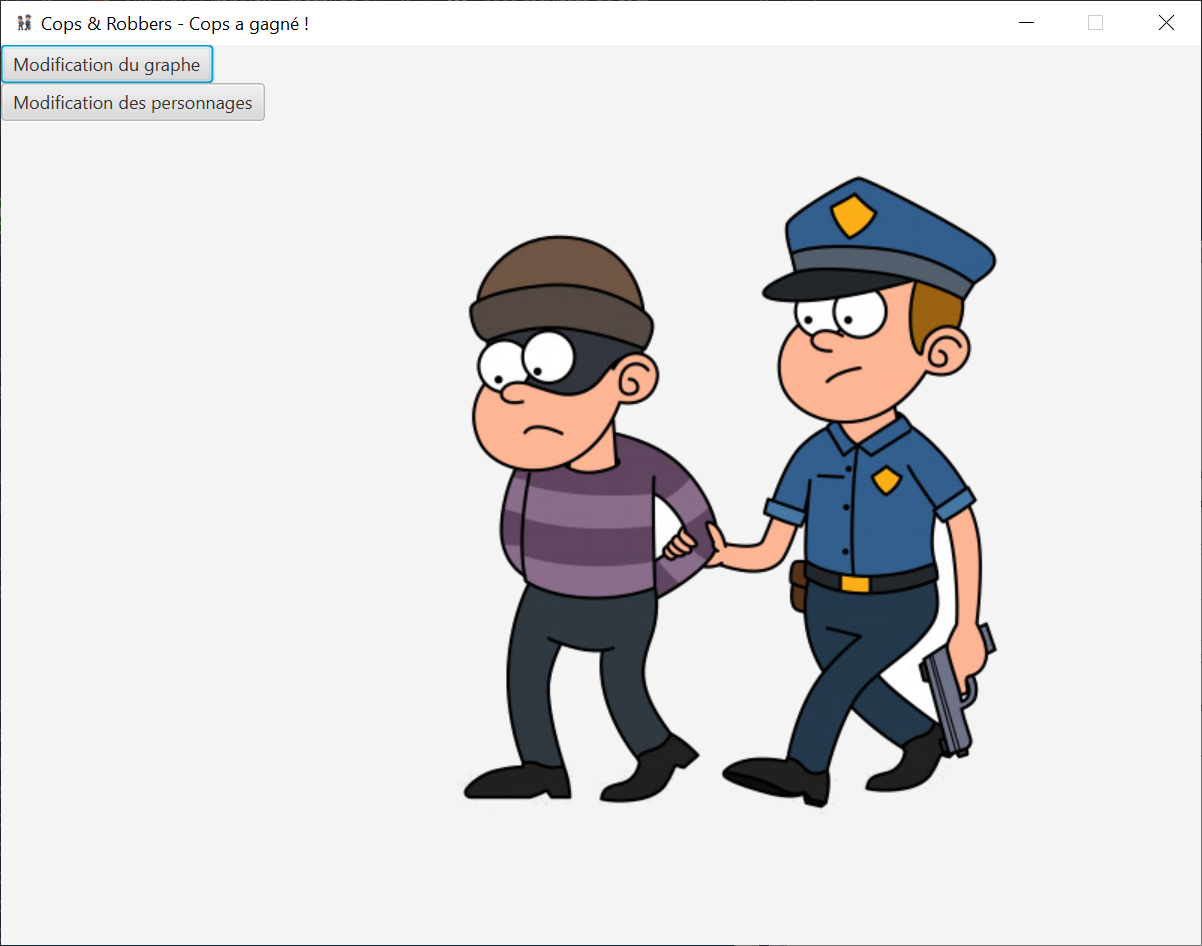
\includegraphics[width=0.45\textwidth]{perdu_fenetre.PNG}}
    \caption{Captures d'écran de mon application}
    \label{fig:screenshots}
\end{figure}

L'application s'ouvre sur une fenêtre (figure \ref{screen:graphe}) où on peut créer des graphes. Grâce à un menu, on peut choisir de créer des noeuds (par clic) et des arêtes (par drag); on peut modifier les noeuds (par drag); et on peut supprimer des noeuds (par clic).

On peut ensuite positionner les personnages, représenter par un éclair gris pour le voleur et un étoile jaune pour les policiers (figure \ref{screen:perso}).

Finalement, on peut jouer aux \cp en déplaçant (par drag) les personnages sur des noeuds voisins (figure \ref{screen:jeu}).

Une fois le voleur attrapé, on a un menu (figure \ref{screen:perdu}) permettant de ré-initialiser le graphe, avec une option pour modifier le graphe (\ref{screen:graphe}) ou réinitialiser les personnages (\ref{screen:perso}).

\section{Discussion}
\subsection{Limitations}

Mon application est fonctionnelle, mais n'a pas encore un visuel attirant. 

Un dernier détail à ajouter est la possibilité de faire vraiment des tours, permettant à l'utilisateur de savoir quel personnage a déjà bougé sur ce tour ci, limittant ainsi les déplacements à une distance de 0 ou 1 pour les policiers et les voleurs alternativement.

J'ai eu un problème de santé qui m'a empêché de faire tout ce que je voulais, notamment l'aspect attractif visuellement de mon application.

\subsection{Bilan et ouverture}

Ce rapport est un résumé de mes recherches dans le domaine des théories des graphes et des jeux sur différentes variantes du problème \cp en particulier sur \hm.

J'ai concentré beaucoup de rigueur à ce rapport, afin qu'il se rapproche d'un article de papier. C'était là le but de mon initiation à la recherche initialement prévue avec Gena Hahn.

Quant à mon application, il est évident qu'elle peut toujours être améliorée. J'ai privilégié la fonctionnalité et la maintenabilité à l'aspect visuel. En effet, le problème de \cp peut facilement être joué et il est facile de modifier le code pour ajouter des fonctionnalités propres aux variantes. Par exemple, il est très facile de permettre aux policiers de ne pas se déplacer uniquement selon les arêtes et ainsi jouer au problème de \hm.

\bibliographystyle{ieeetr}
\bibliography{biblio.bib}


\begin{appendices}
\renewcommand\thesection{Annexe \Alph{section}}
\setcounter{secnumdepth}{1}

\end{appendices}





\end{document}
